\documentclass[xcolor=pdftex,dvipsnames,table,mathserif,aspectratio=169]{beamer}
\usetheme{default}
\usetheme{metropolis}
\usepackage{minted}
\usepackage{mathtools}
\setbeamersize{text margin left=.3in,text margin right=.3in} 

\DeclarePairedDelimiter\abs{\lvert}{\rvert}%
\DeclarePairedDelimiter\norm{\lVert}{\rVert}%

\usepackage[english]{babel}
\usepackage{pgf,pgfarrows,pgfnodes,pgfautomata,pgfheaps}
\usepackage{amsmath,amssymb,setspace,centernot}
\usepackage[latin1]{inputenc}
\usepackage{pgf,tikz}
\usepackage[T1]{fontenc}
\usepackage{relsize}
\usepackage{pdfpages}
\usepackage[absolute,overlay]{textpos} 


\newenvironment{reference}[2]{% 
  \begin{textblock*}{\textwidth}(#1,#2) 
      \footnotesize\it\bgroup\color{red!50!black}}{\egroup\end{textblock*}} 

\DeclareMathSizes{10}{10}{6}{6} 

\begin{document}
\title{Advanced Binary Choice: LPM? Incidental Parameters}
\author{Chris Conlon}
\institute{Panel Data Econometrics}
\date{\today}

\frame{\titlepage}

\section{Intro}

\begin{frame}
\frametitle{Binary Choice: Overview}
Many problems we are interested in look at discrete rather than continuous outcomes.
\begin{itemize}
\item We are familiar with limitations of the linear probability model (LPM)
\begin{itemize}
\item Predictions outside of $[0,1]$
\item Estimates of marginal effects need not be consistent.
\end{itemize}
\item Suppose we have panel data on repeated binary choices
\begin{itemize}
\item When $N$ is large and $T$ is small.
\item Adding FE to the logit/probit model produces biased (and inconsistent) estimates.
\end{itemize}
\item What about the case where $Y$ is binary and a regressor $X$ is endogenous?
\begin{itemize}
\item The usual 2SLS estimator is \alert{NOT consistent}.
\item Or we can ignore the fact that $Y$ is binary...
\item Neither seems like a good option
\end{itemize}
\end{itemize}
\end{frame}

\section*{Problem \#1:\\
 Failures of the LPM}
\begin{frame}
\frametitle{Linear Probability Model}
Consider the LPM with a single continuous regressor
\begin{itemize}
\item LPM prediction departs greatly from CDF long before $[0,1]$ limits.
\item We get probabilities that are too extreme even for $X\hat{\beta}$ ``in bounds''.
\item Some (MHE) argue that though $\hat{Y}$ is flawed, constant marginal effects are still OK.
\end{itemize}
\begin{center}
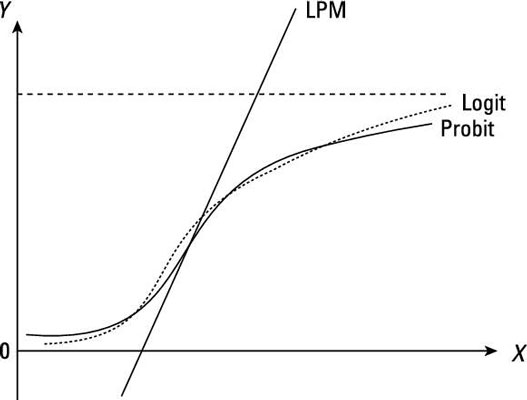
\includegraphics[width=2in]{resources/lpm-probit.jpg}
\end{center}
\end{frame}

\begin{frame}{Some well known textbooks}
(Baby) Wooldrige:
\begin{quote}
``Even with these problems, the linear probability model is useful and often applied in economics. It usually works well for values of the independent variables that are near the averages in the sample.'' (2009, p. 249)
\end{quote}
\begin{itemize}
\item Mentions heteroskedasticity of error (which is binomial given $X$) but does not address the violation of the first LSA.
\end{itemize}
\end{frame}

\begin{frame}{Some well known textbooks}
Angrist and Pischke (MHE) 
\begin{itemize}
\item several examples where marginal effects of probit and LPM are ``indistinguishable''.
\end{itemize}

\begin{quote}
...while a nonlinear model may fit the CEF (conditional expectation function) for LDVs (limited dependent variable models) more closely than a linear model, when it comes to marginal effects, this probably matters little. This optimistic conclusion is not a theorem, but as in the empirical example here, it seems to be fairly robustly true.(2009, p. 107)
\end{quote}
and continue...
\begin{quote}
...extra complexity comes into the inference step as well, since we need standard errors for marginal effects. (ibid.)
\end{quote}
\end{frame}

\begin{frame}
\frametitle{Linear Probability Model}
How does the LPM work?
\begin{eqnarray*}
D = X \beta + \varepsilon
\end{eqnarray*}
\begin{itemize}
\item Estimated $\hat{\beta}$ are the MFX.
\item With exogenous $X$ we have $E[D | X] = Pr[D=1 | X] = X \beta$.
\item If some elements of $X$ (including treatment indicators) are endogenous or mismeasured they will be correlated with $\varepsilon$.
\item In that case we can do IV via 2SLS or IV-GMM given some instruments $Z$.
\end{itemize}
\end{frame}


\begin{frame}
\frametitle{Linear Probability Model}
\begin{eqnarray*}
D = X \beta + \varepsilon
\end{eqnarray*}
\begin{itemize}
\item We need the usual $E[\varepsilon  | X]= 0 $ or $E[\varepsilon | Z] = 0$.
\item An obvious flaw: Given any $\varepsilon | X  $ must equal either $1- X \beta$ or $-X \beta$ which are functions of $X$
\item \alert{Only the trivial binary $X$ with no other regressors satisfies this!}
\item Should you believe $\widehat{\beta}_{LPM}$ if $E[\varepsilon | X ] \neq 0$?
\end{itemize}
\end{frame}

\begin{frame}
\frametitle{Alarming Example: Lewbel Dong and Yang (2012)}
\begin{itemize}
\item LPM is not just about taste and convenience.
\item Three treated observations, three untreated % \texttt{Treated=1}
\item Assume that $f(\varepsilon) \sim N(0,\sigma^2)$
\begin{eqnarray*}
D = I ( 1 + Treated + R + \varepsilon \geq 0 ) 
\end{eqnarray*}
\item Each individual treatment effect given by:
\begin{eqnarray*}
 I ( 2 + R + \varepsilon \geq 0 ) -  I ( 1 + R + \varepsilon \geq 0 )  =  I ( 0 \leq 1 + R + \varepsilon \leq 1 ) 
\end{eqnarray*}
\item All treatment effects are positive for all $(R,\varepsilon)$.
\item Construct a sample where true effect $=1$ for 5th individual, 0 otherwise. $ATE= \frac{1}{6}$.
\end{itemize}
\end{frame}

\begin{frame}[fragile]
\frametitle{Alarming Example: Lewbel Dong and Yang (2012)}
For stable draws -- I chose the outcome $D$:
\begin{verbatim}
draw_sample = function(){
  tibble(
  r = c(-1.8, -0.9, -0.92,-2.1, -1.92, 10),
  treated = c(0,0,0,1,1,1),
  true_te = c(0,0,0,0,1,0),
  error = rnorm(6),
  D = c(0,1,1,0,1,1)
  )  %>% mutate(y = (r + true_te * treated + error)>0) 
  }
\end{verbatim}
\end{frame}


\begin{frame}[fragile]
\frametitle{Alarming Example: Lewbel Dong and Yang (2012)}
\begin{verbatim}
  lm(D~ treated+r, data=fake_data)
  
Coefficients:
             Estimate Std. Error t value Pr(>|t|)    
(Intercept)  0.725146   0.008016   90.46   <2e-16 ***
treated     -0.155084   0.011938  -12.99   <2e-16 ***
r            0.048464   0.001381   35.09   <2e-16 ***
\end{verbatim}
\end{frame}

\begin{frame}[fragile]{A Small Sample Issue ?}
\begin{verbatim}
# Now with 1000x more data
for (n in 1:1000){data[[n]]=draw_sample()}
df<-bind_rows(data)
summary(lm(y~ treated+r, data=df))


Coefficients:
             Estimate Std. Error t value Pr(>|t|)    
(Intercept) 0.2364993  0.0055112   42.91   <2e-16 ***
treated     0.0055820  0.0082069    0.68    0.496    
r           0.0763806  0.0009495   80.44   <2e-16 ***
\end{verbatim}

\end{frame}


\begin{frame}[fragile]
\frametitle{Alarming Example: Lewbel Dong and Yang (2012)}
\begin{itemize}
\item That went well, except that:
\begin{itemize}
\item we got the wrong sign of $\beta_T$
\item $\beta_1/\beta_2$ was the wrong sign and three times too big.
\end{itemize}
\item this is not because of small sample size or $\beta_1 \approx 0$.
\item As $n \rightarrow \infty$ we can get an arbitrarily precise wrong answer.
\item We don't even get the sign right!
\item This is still in OLS (not much hope for 2SLS).
\end{itemize}
\tiny

\end{frame}


\section*{Problem \#2:\\
Incidental Parameters Problem}

\begin{frame}
\frametitle{Problem \#2: Fixed Effects and Incidental Parameters}
Threshold Crossing / Latent Variable Model:
\begin{eqnarray*}
y_{it} = \mathbf{1}(X_{it} \beta + \epsilon_{it} \geq 0)
\end{eqnarray*}
Individuals $i=1,\ldots,N$, and periods $t=1,\ldots,T$.
\begin{itemize}
\item  Goal is not usually $\hat{\beta}$ or it's CI
\item Instead  $P(y_{it}=1 | x_{it})$ or $\frac{\partial P[y_{it}=1 | x_{it}] }{\partial x_{it}}$ (marginal effects).
\end{itemize}
What about if we want to add FE $\alpha_i$?
\begin{eqnarray*}
y_{it} = \mathbf{1}(X_{it} \beta +\alpha_i+ \epsilon_{it} \geq 0)
\end{eqnarray*}
Best case scenario $E[\epsilon_{it} | x_{i1} ,\ldots, x_{iT}, \alpha_i]=0$.
\end{frame}


\begin{frame}
\frametitle{ Fixed Effects and Incidental Parameters}
Let's try and difference out (within transform) the FE:
\begin{eqnarray*}
E[y_{it}-y_{i,t-1} | X_i,\alpha_i] =E[F(X_{i,t} \beta +\alpha_i)- F(X_{i,t-1} \beta +\alpha_i) | X_i]
\end{eqnarray*}
\begin{itemize}
\item We can't difference out the FE anymore!
\item $\alpha_i$ doesn't have the interpretation as $\overline{y}_i$.
\item The effect of $\alpha_i$ will now depend on $X_{i,t}$.
\item We need to estimate $N$ parameters $\alpha_1, \ldots,\alpha_N$.
\end{itemize}
\end{frame}

\begin{frame}
\frametitle{ Fixed Effects and Incidental Parameters}
\begin{itemize}
\item FE requires maximizing $LL$ over $(\alpha_i,\beta)$.
\item FE model inconsistent as $N\rightarrow \infty$ as $T$ fixed.
\item Under OLS we have a \alert{consistent estimator} of $\alpha_i$, as $N$ gets big, random noise in $\alpha_i$ washes out.
\item Under Logit/Probit/etc. now we only have $T$ observations.
\item Under logit/probit bias in $\hat{\beta}$ can be pretty bad.
\item Under probit, bias in \alert{marginal effects} tends not to be as bad as bias in $\hat{\beta}$ (Hahn and Newey, 2004).
\end{itemize}
\end{frame}


\begin{frame}
\frametitle{ Fixed Effects and Incidental Parameters}
\begin{align*}
Pr(y_{it}=1 | z_{it}) &= \frac{\exp(z_{it} )}{1+\exp(z_{it})}\\
z_{it} &= x_{it} + \alpha_i + u_{it}\\
x_{it} &=  \alpha_i + v_{it}
\end{align*}
Generate data from a binary logit with some simple FE.
\begin{itemize}
\item $\alpha_i \sim N(0,1)$
\item $v_{it} \sim N(0,1)$
\item $u_{it} \sim N(0,2)$
\end{itemize}
\end{frame}

\begin{frame}[fragile]{How bad is it? An example}
\scriptsize
\begin{verbatim}
library(fabricatr)
fe.sd <- 1 # Specify the standard deviation of the fixed effed
x.sd  <- 1 # Specify the base standard deviation of x
nperson <- 5000 # Number of persons
nobs <- 5      # Number of observations per person
panels <- fabricate(
  individuals = add_level(N = nperson, id_fe = rnorm(N,0,fe.sd)),
  periods = add_level(N = nobs, nest = FALSE),
  obs = cross_levels(
    by = join(individuals, periods),
    # put the FE into X so there is something to de-mean
    x = id_fe + rnorm(N,0,x.sd),
    z = 1*id_fe  + 1*x, # + rnorm(N,0,1) -- adding this breaks bias correction
    logit_prob = exp(z)/(1+exp(z)),
    yl= logit_prob>runif(N)
  )
)
\end{verbatim}
\end{frame}


\begin{frame}[fragile]{How bad is it? An example}
\scriptsize
\begin{semiverbatim}
summary(glm(yl ~ x, data = panels, family = "binomial"))

Coefficients:
              Estimate Std. Error z value Pr(>|z|)    
(Intercept) -0.0002284  0.0162293  -0.014    0.989    
x            \alert{1.4135577}  0.0181815  77.747   <2e-16 ***

summary(glm(yl ~ x+factor(id_fe), data = panels, family = "binomial"))
Estimates:
  Estimate Std. error z value Pr(> |z|)    
x  \alert{1.36383}    0.02852   47.82    <2e-16 ***
...
\end{semiverbatim}
The latter takes 10+ minutes and often FE make things worse.
\end{frame}

\begin{frame}{Two Solutions}
Two possible solutions:
\begin{enumerate}
\item Work out an analytic expression for the bias and subtract it off: \alert{analytic bias correction}.
\item Conditional Logit. Exploit a \alert{sufficient statistic} formulation (Chamberlain)
\end{enumerate}
\end{frame}


\begin{frame}{Approach \#1: Estimate the FE, Fix the Bias }
What does \texttt{bife} do?
\begin{itemize}
\item Estimate the model with the FE in there as parameters (dummy variables).
\item This model is \alert{biased} and \alert{inconsistent}.
\item It is a big pain to estimate if $N$ becomes large (lots of parameters, lots of derivatives, etc.)
\begin{itemize}
\item Exploits the \alert{sparsity} of the Hessian, much faster than \texttt{glm}
\end{itemize}
\item Fix the bias on the back end by working out an analytic expression or jackknife: Hahn and Newey (2004) or Stammann,  Heiss, and McFadden (2016).
\end{itemize}
\end{frame}

\begin{frame}[fragile]{\texttt{bife} First the inconsistent model}
\scriptsize
\begin{semiverbatim}
res<-bife(yl ~ x | id_fe, data = panels, 'logit')

binomial - logit link

yl ~ x | id_fe

Estimates:
  Estimate Std. error z value Pr(> |z|)    
x  \alert{1.36383}    0.02852   47.82    <2e-16 ***
---
Signif. codes:  0 ?***? 0.001 ?**? 0.01 ?*? 0.05 ?.? 0.1 ? ? 1

residual deviance= 15933.43,
null deviance= 22929.24,
nT= 16540, N= 3308

( 8460 observation(s) deleted due to perfect classification )

...
\end{semiverbatim}
\end{frame}


\begin{frame}[fragile]{\texttt{bife} Analytic Bias Correction (Ex-post)}
\scriptsize
\begin{semiverbatim}
> summary(bias_corr(res))
binomial - logit link

yl ~ x | id_fe

Estimates:
  Estimate Std. error z value Pr(> |z|)    
x  \alert{1.02455}    0.02483   41.26    <2e-16 ***
---
Signif. codes:  0 ?***? 0.001 ?**? 0.01 ?*? 0.05 ?.? 0.1 ? ? 1

residual deviance= 16089.15,
null deviance= 22929.24,
nT= 16540, N= 3308

( 8460 observation(s) deleted due to perfect classification )

Number of Fisher Scoring Iterations: 5 


\end{semiverbatim}
\end{frame}




\begin{frame}{Conditional MLE}
Imagine a sufficient statistic $S_i$:
\begin{align*}
f\left(Y_{i} | X_{i}, S_{i}, \theta, \alpha_{i}\right)=f\left(Y_{i} | X_{i}, S_{i}, \theta\right)\\
\hat{\theta}=\arg \max _{\theta} \sum_{i=1}^{n} f\left(Y_{i} | X_{i}, S_{i}, \theta\right)
\end{align*}
These are hard to find, but examples:
\begin{itemize}
\item Binary Logit
\item Gaussian linear model
\item Poisson
\item (and as we have seen) PH model for durations
\end{itemize}
\end{frame}




\begin{frame}{Conditional Logit  (Chamberlain 1984/1992)} 
Here $S_i = \sum_{t} y_{it}$. Assume that $T=2$ to make things clear
\begin{align*}
E[y_{i1} | X_i, \alpha_i, y_{i1}+y_{i2}=1]
\end{align*}
Consider the $\sum_{t} y_{it}=1$ case:
\begin{align*}
\operatorname{Pr}\left(\mathrm{y}_{\mathrm{i} 1}+\mathrm{y}_{\mathrm{i} 2}=1\right)=\operatorname{Pr}\left(\mathrm{y}_{\mathrm{i} 1}=0, \mathrm{y}_{\mathrm{i} 2}=1\right)+\operatorname{Pr}\left(\mathrm{y}_{\mathrm{i} 1}=1, \mathrm{y}_{\mathrm{i} 2}=0\right)
\end{align*}
And then we can write:
\begin{align*}
\operatorname{Pr}\left(\mathrm{y}_{\mathrm{i} 1}=1\right) \quad&=\quad \exp \left(\alpha_i+\mathrm{x}_{\mathrm{it}}^{\prime} \beta\right) /\left[1+\exp \left(\alpha_i+\mathrm{x}_{\mathrm{it}}^{\prime} \beta\right)\right]\\
\operatorname{Pr}\left(\mathrm{y}_{\mathrm{i} 1}=0\right) \quad&=\quad 1-\exp \left(\alpha_i+\mathrm{x}_{\mathrm{it}}^{\prime} \beta\right) /\left[1+\exp \left(\alpha_i+\mathrm{x}_{\mathrm{it}}^{\prime} \beta\right)\right]\\
&=1 /\left[1+\exp \left(\alpha_i+\mathrm{x}_{\mathrm{it}}^{\prime} \beta\right)\right]
\end{align*}
\end{frame}

\begin{frame}{Conditional Logit  (Chamberlain 1984/1992)}
\footnotesize
\begin{align*}
\operatorname{Pr}\left(\mathrm{y}_{\mathrm{i} 1}=1, \mathrm{y}_{\mathrm{i} 2}=0\right) &= 
\frac{\exp \left(\alpha_i+\mathrm{x}_{\mathrm{i} 1}^{\prime} \beta\right)}{1+\exp \left(\alpha_i+\mathrm{x}_{\mathrm{i} 1}^{\prime} \beta\right)} \cdot \frac{1}{1+\exp \left(\alpha_i+\mathrm{x}_{\mathrm{i} 2}^{\prime} \beta\right)}\\
\operatorname{Pr}\left(\mathrm{y}_{\mathrm{i} 1}=0, \mathrm{y}_{\mathrm{i} 2}=1\right) &=
 \frac{1}{1+\exp \left(\alpha_i+\mathrm{x}_{\mathrm{i} 1}^{\prime} \beta\right)} \cdot \frac{\exp \left(\alpha_i+\mathrm{x}_{\mathrm{i} 2}^{\prime} \beta\right)}{1+\exp \left(\alpha_i+\mathrm{x}_{\mathrm{i} 2}^{\prime} \beta\right)}
\end{align*}
Putting it together
\begin{align*}
\operatorname{Pr}\left(\mathrm{y}_{\mathrm{i} 1}+\mathrm{y}_{\mathrm{i} 2}=1\right) \quad=\operatorname{Pr}\left(\mathrm{y}_{\mathrm{i} 1}=0, \mathrm{y}_{\mathrm{i} 2}=1\right)+\operatorname{Pr}\left(\mathrm{y}_{\mathrm{i} 1}=1, \mathrm{y}_{\mathrm{i} 2}=0\right)\\
=\frac{\exp \left(\alpha_i+\mathrm{x}_{\mathrm{i} 1}^{\prime} \beta\right)+\exp \left(\alpha_i+\mathrm{x}_{\mathrm{i} 2}^{\prime} \beta\right)}{\left(1+\exp \left(\alpha_i+\mathrm{x}_{\mathrm{il}}^{\prime} \beta\right)\right)\left(1+\exp \left(\alpha_i + \mathrm{x}_{\mathrm{i} 2}^{\prime} \beta\right)\right)}
\end{align*}
And the conditional:
\begin{align*}
\operatorname{Pr}\left(\mathrm{y}_{\mathrm{i} 1}=1, \mathrm{y}_{\mathrm{i} 2}=0 | \mathrm{y}_{\mathrm{i} 1}+\mathrm{y}_{\mathrm{i} 2}=1\right) \quad=\quad \frac{\operatorname{Pr}\left(\mathrm{y}_{\mathrm{i} 1}=1, \mathrm{y}_{\mathrm{i} 2}=0\right)}{\operatorname{Pr}\left(\mathrm{y}_{\mathrm{i} 1}+\mathrm{y}_{\mathrm{i} 2}=1\right)}\\
\frac{\exp \left(\alpha_i+\mathrm{x}_{\mathrm{i} 1}^{\prime} \beta\right)}{\exp \left(\alpha_i+\mathrm{x}_{\mathrm{i} 1}^{\prime} \beta\right)+\exp \left(\alpha_i+\mathrm{x}_{\mathrm{i} 2}^{\prime} \beta\right)}=\frac{\exp \left(\mathrm{x}_{\mathrm{i} 1}^{\prime} \beta\right)}{\exp \left(\mathrm{x}_{\mathrm{i} 1}^{\prime} \beta\right)+\exp \left(\mathrm{x}_{\mathrm{i} 2}^{\prime} \beta\right)}
\end{align*}
\end{frame}

\begin{frame}{Eliminating the FE (Chamberlain 1984/1992)}
Notice that we've now eliminated the FE!
\begin{align*}
\operatorname{Pr}\left(\mathrm{y}_{\mathrm{i} 1}=1, \mathrm{y}_{\mathrm{i} 2}=0 | \mathrm{y}_{\mathrm{i} 1}+\mathrm{y}_{\mathrm{i} 2}=1\right)&=
\frac{1}{1+\exp \left(\mathrm{x}_{\mathrm{i} 2}-\mathrm{x}_{\mathrm{i} 1}\right)^{\prime} \beta}\\
\operatorname{Pr}\left(\mathrm{y}_{\mathrm{i} 1}=1, \mathrm{y}_{\mathrm{i} 2}=0 | \mathrm{y}_{\mathrm{i} 1}+\mathrm{y}_{\mathrm{i} 2}=1\right)&=
\frac{\exp \left(\mathrm{x}_{\mathrm{i} 2}-\mathrm{x}_{\mathrm{i} 1}\right)^{\prime} \beta}{1+\exp \left(\mathrm{x}_{\mathrm{i} 2}-\mathrm{x}_{\mathrm{i} 1}\right)^{\prime} \beta}
\end{align*}
\begin{itemize}
\item As per usual if $x_{it}$ doesn't vary over $t$ it drops out too.
\item We can skip the $y_{i1} + y_{i2}=2$ and $y_{i1} + y_{i2}=0$ case, why?
\begin{itemize}
\item The FE $\alpha_i \rightarrow \pm \infty$
\end{itemize}
\end{itemize}
\end{frame}


\begin{frame}[fragile]{In practice \texttt{clogit} in R }
\begin{semiverbatim}
library(survival)
> summary(clogit(yl~ x +strata(id_fe), data=panels))
Call:
coxph(formula = Surv(rep(1, 25000L), yl) ~ x + strata(id_fe), 
    data = panels, method = "exact")

  n= 25000, number of events= 12517 

     coef exp(coef) se(coef)     z Pr(>|z|)    
x \alert{1.04162}   2.83381  0.02405 43.31   <2e-16 ***
\end{semiverbatim}
\end{frame}
\section*{Thanks!}

\end{document}
